\chapter{Replicación del ADN y mitosis}\label{ch:b1:replication-mitosis}

Cada ocho horas aproximadamente, una \omterm{def:b1:cell-unit-of-life:cell}{célula} del revestimiento intestinal
copia seis mil millones de \omterm{thm:b1:nucleic-acids:helix}{pares de bases} con alrededor de un error por cada
mil millones, y reparte después las dos copias entre dos hijas de modo que
cada una reciba exactamente cuarenta y seis \omterm{def:b1:genomes:genome}{cromosomas}: ni cuarenta y cinco,
ni cuarenta y siete. La copia la hace una máquina que lee una hebra y
construye su complementaria a cincuenta letras por segundo desde decenas de
miles de puntos de partida a la vez; el reparto lo hace un \omterm{def:b1:replication-mitosis:mitosis}{huso} de
\omterm{def:b1:eukaryotic-cell:cytoskeleton}{microtúbulos} que separa las dos copias de cada \omterm{def:b1:genomes:genome}{cromosoma} con una precisión
de un error por cada cien mil divisiones. Este capítulo describe la
\omterm{def:b1:replication-mitosis:fork}{horquilla de replicación} y sus \omterm{def:b1:enzymes:enzyme}{enzimas}, el problema de los extremos, el
\omterm{def:b1:replication-mitosis:cycle}{ciclo celular} que marca los tiempos de la replicación y la división, y la
\omterm{def:b1:replication-mitosis:mitosis}{mitosis}, que es la división misma.

\section{Replicación semiconservativa}

\begin{proposition}[Cada hebra es un molde]\label{prop:b1:replication-mitosis:semiconservative}
\index{replicación semiconservativa}
El \omterm{def:b1:nucleic-acids:chain}{ADN} se replica de forma \emph{semiconservativa}: las dos hebras de la
hélice se separan y cada una sirve de molde sobre el que se construye una
hebra complementaria nueva, de modo que toda molécula hija es una hebra
vieja apareada con una nueva.
\end{proposition}
\begin{proof}[Evidencia]
Meselson y Stahl (1958; recordado del volumen de bachillerato) cultivaron
\emph{E. coli} con nitrógeno pesado, la transfirieron a nitrógeno ligero y
separaron el \omterm{def:b1:nucleic-acids:chain}{ADN} por densidad: tras una generación todo el \omterm{def:b1:nucleic-acids:chain}{ADN} era de
densidad intermedia y, tras dos, la mitad intermedia y la mitad ligera:
exactamente lo que predice una hebra vieja y otra nueva por molécula, y
ningún otro esquema. Cairns (1963) marcó con tritio \omterm{def:b1:genomes:genome}{cromosomas} bacterianos
en replicación y los fotografió por autorradiografía: círculos con una
``burbuja'' de replicación cuyas dos horquillas se alejaban en sentidos
opuestos desde un único origen. Kornberg (1956) purificó una \omterm{def:b1:enzymes:enzyme}{enzima} que
sintetizaba \omterm{def:b1:nucleic-acids:chain}{ADN} en el tubo de ensayo a partir de los cuatro nucleósidos
trifosfato y un molde, siguiendo la secuencia del molde.
\end{proof}

\begin{definition}[La horquilla de replicación y sus enzimas]\label{def:b1:replication-mitosis:fork}
\index{horquilla de replicación}\index{ADN polimerasa}\index{fragmento de Okazaki}
La replicación empieza en un \emph{origen} --- uno en el \omterm{def:b1:genomes:genome}{cromosoma}
bacteriano, decenas de miles en un \omterm{def:b1:genomes:genome}{genoma} eucariota ---, donde la hélice se
abre y dos \emph{horquillas de replicación} se alejan en sentidos opuestos.
En cada horquilla: una \emph{helicasa} desenrolla la hélice (un \omterm{def:b1:water-small-molecules:atp}{ATP} por \omterm{thm:b1:nucleic-acids:helix}{par
de bases}), unas \emph{\omterm{def:b1:proteins:peptide}{proteínas} de unión a hebra sencilla} mantienen
separadas las hebras y una \emph{topoisomerasa} situada por delante de la
horquilla libera la torsión que el desenrollamiento acumula. La \emph{\omterm{def:b1:nucleic-acids:chain}{ADN}
polimerasa} añade \omterm{def:b1:nucleic-acids:nucleotide}{nucleótidos} solo al hidroxilo $3'$ de una cadena ya
existente, de modo que toda hebra nueva crece de $5' \to 3'$ y ninguna puede
empezar de la nada: una \emph{primasa} coloca primero un \emph{cebador}
corto de \omterm{def:b1:nucleic-acids:chain}{ARN} que la polimerasa alarga. Sobre el molde que se lee de
$3' \to 5'$, la hebra nueva crece de forma continua hacia la horquilla: es
la \emph{hebra conductora}. Sobre el otro molde, la hebra nueva debe crecer
alejándose de la horquilla, en trozos de \qtyrange{1000}{2000}{} \omterm{def:b1:nucleic-acids:nucleotide}{nucleótidos}
en las bacterias y de \qtyrange{100}{200}{} en los eucariotas, los
\emph{fragmentos de Okazaki}, cada uno con su propio cebador: es la
\emph{hebra retardada}. Una segunda polimerasa sustituye los cebadores por
\omterm{def:b1:nucleic-acids:chain}{ADN} y una \emph{ligasa} sella los fragmentos en una sola hebra.
\end{definition}

\begin{omfigure}
\begin{tikzpicture}[font=\footnotesize, >=Stealth, line cap=round]
  % parental duplex on the right, opening leftward
  \draw[very thick, omDef] (12.4,1.0) -- (7.6,1.0);
  \draw[very thick, omDef!50] (12.4,-1.0) -- (7.6,-1.0);
  \foreach \x in {8.0,8.6,...,12.2} { \draw[thick, gray!60] (\x,1.0) -- (\x,-1.0); }
  \node[anchor=south] at (10.0,1.15) {dúplex parental};
  % helicase at the fork
  \node[circle, draw, thick, fill=omProp!40, minimum size=9mm, font=\scriptsize] (hel) at (7.3,0) {helicasa};
  \draw[->, very thick, omProp!80!black] (6.4,-1.9) -- (5.2,-1.9) node[left, font=\scriptsize] {avanza la horquilla};
  % separated template strands going left
  \draw[very thick, omDef] (7.0,0.55) .. controls (5.5,1.5) .. (0.4,2.2);
  \draw[very thick, omDef!50] (7.0,-0.55) .. controls (5.5,-1.5) .. (0.4,-2.2);
  \node[anchor=east, omDef] at (0.3,2.2) {$3'$};
  \node[anchor=east, omDef!70!black] at (0.3,-2.2) {$5'$};
  % leading strand: continuous new strand along upper template
  \draw[very thick, omThm] (1.0,1.85) .. controls (4.5,1.35) .. (6.2,0.75);
  \node[draw, thick, fill=omThm!25, rounded corners=3pt, inner sep=2pt, font=\scriptsize] at (6.0,0.95) {pol};
  \node[anchor=south west, omThm, align=left] at (1.0,2.35) {hebra conductora: continua, de $5' \to 3'$ hacia la horquilla};
  \node[anchor=east, omThm] at (0.95,1.85) {$5'$};
  % lagging strand: Okazaki fragments along lower template, each with a primer
  \foreach \x/\y in {1.2/-1.95, 3.3/-1.55, 5.3/-1.05} {
    \fill[omExo!80!black] (\x,\y) circle (0.08);
    \draw[very thick, omThm] (\x,\y) .. controls (\x+0.8,\y+0.15) .. (\x+1.5,\y+0.25);
  }
  \node[draw, thick, fill=omThm!25, rounded corners=3pt, inner sep=2pt, font=\scriptsize] at (6.7,-1.0) {pol};
  \node[anchor=north west, align=left] at (1.0,-2.5) {hebra retardada: fragmentos de Okazaki, cada uno iniciado por un cebador de ARN (\textcolor{omExo!80!black}{punto}),\\ que crecen de $5' \to 3'$ alejándose de la horquilla; los cebadores se sustituyen y la ligasa une los fragmentos};
  \node[font=\scriptsize, anchor=south] at (3.3,-1.35) {$5'$};
\end{tikzpicture}

{\small Una \omterm{def:b1:replication-mitosis:fork}{horquilla de replicación}. La helicasa abre el dúplex parental;
la hebra conductora se copia de forma continua hacia la horquilla y la
retardada hacia atrás, en \omterm{def:b1:replication-mitosis:fork}{fragmentos de Okazaki}, porque las polimerasas solo
construyen en el sentido $5' \to 3'$.}
\end{omfigure}

\begin{proposition}[Fidelidad]\label{prop:b1:replication-mitosis:fidelity}
\index{corrección de pruebas}
El apareamiento de bases por sí solo daría alrededor de un error por cada
$10^5$; la polimerasa \emph{corrige} --- una actividad exonucleasa
$3' \to 5'$ retira un \omterm{def:b1:nucleic-acids:nucleotide}{nucleótido} mal apareado antes de añadir el
siguiente --- y lleva el error a uno por cada $10^7$; y después de que pase
la horquilla, un sistema de \emph{reparación de desapareamientos} encuentra
los desapareamientos restantes, identifica la hebra nueva y la corrige: un
error por cada $10^9$ o $10^{10}$ \omterm{thm:b1:nucleic-acids:helix}{pares de bases} replicados. Una \omterm{def:b1:cell-unit-of-life:cell}{célula}
humana que copia $\num{6.4e9}$ pares comete un puñado de mutaciones cada vez
que se divide; una bacteria, una cada mil divisiones.
\end{proposition}

\begin{example}[Velocidad y puntos de partida]\label{ex:b1:replication-mitosis:speed}
Una horquilla bacteriana avanza a \qty{1000}{} \omterm{thm:b1:nucleic-acids:helix}{pares de bases} por segundo:
dos horquillas copian los \qty{4.6}{Mb} de \emph{E. coli} en \qty{40}{min}
y, en un medio rico donde la \omterm{def:b1:cell-unit-of-life:cell}{célula} se divide cada veinte, una ronda nueva
empieza antes de que termine la anterior. Una horquilla eucariota, frenada
por la cromatina, avanza a \qty{50}{} por segundo: copiar un \omterm{def:b1:genomes:genome}{cromosoma}
humano de \qty{250}{Mb} desde un solo origen llevaría un mes, así que el
\omterm{def:b1:genomes:genome}{genoma} se copia desde unos \num{40000} orígenes en ocho horas, en un orden
fijo para cada tipo celular.
\end{example}

\section{Los extremos}

\begin{proposition}[El problema de la replicación de los extremos y la telomerasa]\label{prop:b1:replication-mitosis:telomerase}
\index{telomerasa}
En un \omterm{def:b1:genomes:genome}{cromosoma} lineal, la hebra retardada no puede completarse hasta el
extremo mismo: al retirarse el último cebador no hay ningún hidroxilo $3'$
aguas arriba desde el que rellenar el hueco, y cada replicación acortaría el
\omterm{def:b1:genomes:genome}{cromosoma} en \qtyrange{50}{100}{} \omterm{def:b1:nucleic-acids:nucleotide}{nucleótidos}. Los eucariotas terminan sus
\omterm{def:b1:genomes:genome}{cromosomas} con \emph{\omterm{def:b1:genomes:karyotype}{telómeros}}, miles de copias de una repetición corta
(TTAGGG en los vertebrados) que no llevan \omterm{def:b1:genomes:gene}{genes}, y las \omterm{def:b1:cell-unit-of-life:cell}{células} germinales y
las \omterm{def:b1:cell-unit-of-life:cell}{células} madre poseen \emph{telomerasa}, una \omterm{def:b1:enzymes:enzyme}{enzima} con su propio molde
de \omterm{def:b1:nucleic-acids:chain}{ARN} que añade repeticiones al extremo $3'$ y repone lo que la replicación
pierde. Casi todas las \omterm{def:b1:cell-unit-of-life:cell}{células} somáticas carecen de ella: sus \omterm{def:b1:genomes:karyotype}{telómeros} se
acortan en cada división y, tras unas cincuenta divisiones en cultivo, dejan
de dividirse. Las bacterias, con \omterm{def:b1:genomes:genome}{cromosomas} circulares, no tienen extremos.
\end{proposition}

\begin{omfigure}
\begin{tikzpicture}[font=\footnotesize, >=Stealth, line cap=round]
  % top: the problem
  \draw[very thick, omDef] (0,1.2) -- (8,1.2) node[right] {$3'$ (molde)};
  \draw[very thick, omThm] (0,0.8) -- (6.3,0.8);
  \fill[omExo!80!black] (6.3,0.8) circle (0.08); \draw[very thick, omExo!80!black] (6.3,0.8) -- (7.0,0.8);
  \node[anchor=east, omThm] at (-0.1,0.8) {hebra retardada nueva $5'$};
  \node[anchor=north, font=\scriptsize, omExo!80!black] at (6.65,0.72) {último cebador};
  \draw[thick, gray] (7.0,0.55) -- (8.0,0.55);
  \node[anchor=north, font=\scriptsize, align=center, gray] at (7.5,0.45) {hueco: nada desde donde alargar\\ una vez retirado el cebador};
  % bottom: telomerase
  \draw[very thick, omDef] (0,-1.6) -- (8,-1.6);
  \draw[very thick, omDef, dashed] (8,-1.6) -- (10.2,-1.6) node[right] {$3'$ alargado};
  \node[draw, thick, fill=omProp!30, rounded corners=4pt, inner sep=3pt, align=center, font=\scriptsize] at (9.1,-0.95) {telomerasa\\ (con molde de ARN dentro)};
  \draw[very thick, omThm] (0,-2.0) -- (6.3,-2.0);
  \draw[very thick, omThm, dashed] (6.3,-2.0) -- (8.6,-2.0);
  \node[anchor=east, align=right, font=\scriptsize] at (-0.1,-1.8) {repeticiones teloméricas\\ TTAGGG\ldots};
  \node[anchor=north, align=center, gray] at (5,-2.3) {la telomerasa alarga con repeticiones el extremo $3'$ del molde; un cebador nuevo sobre\\ esa prolongación permite completar la hebra retardada hasta la longitud original};
\end{tikzpicture}

{\small El problema de la replicación de los extremos (arriba) y su
solución (abajo). La hebra retardada queda corta en el extremo del
\omterm{def:b1:genomes:genome}{cromosoma}; la telomerasa añade repeticiones al extremo $3'$ del molde para
que la pérdida recaiga en secuencia que no lleva \omterm{def:b1:genomes:gene}{genes}.}
\end{omfigure}

\section{El ciclo celular}

\begin{definition}[El ciclo celular]\label{def:b1:replication-mitosis:cycle}
\index{ciclo celular}\index{interfase}
El \emph{ciclo celular} de una \omterm{def:b1:cell-unit-of-life:prokeuk}{célula eucariota} tiene cuatro fases.
\emph{G$_1$} (intervalo 1): la \omterm{def:b1:cell-unit-of-life:cell}{célula} crece y fabrica las \omterm{def:b1:enzymes:enzyme}{enzimas} de la
replicación; \emph{S} (síntesis): replica su \omterm{def:b1:nucleic-acids:chain}{ADN}, de modo que cada \omterm{def:b1:genomes:genome}{cromosoma}
pasa a ser dos \emph{\omterm{def:b1:replication-mitosis:mitosis}{cromátidas} hermanas} idénticas unidas por el
\omterm{def:b1:genomes:karyotype}{centrómero}; \emph{G$_2$}: sigue creciendo y comprueba las copias; \emph{M}:
la \emph{\omterm{def:b1:replication-mitosis:mitosis}{mitosis}}, la división del núcleo, seguida de la
\emph{citocinesis}, la división del \omterm{def:b1:cell-unit-of-life:cell}{citoplasma}. G$_1$, S y G$_2$ juntas son
la \emph{interfase}, en la que los \omterm{def:b1:genomes:genome}{cromosomas} están extendidos y activos;
una \omterm{def:b1:cell-unit-of-life:cell}{célula} que deja de dividirse abandona el ciclo desde G$_1$ hacia un
estado de reposo, G$_0$. Una \omterm{def:b1:cell-unit-of-life:cell}{célula} humana en división tarda alrededor de
\qty{24}{h}: G$_1$ \qty{10}{h}, S \qty{8}{h}, G$_2$ \qty{4}{h}, M
\qty{1}{h}; una levadura, \qty{90}{min}; y un embrión temprano de rana,
treinta minutos sin intervalo alguno.
\end{definition}

\begin{omfigure}
\begin{tikzpicture}
\begin{axis}[
  width=0.9\linewidth, height=5.6cm,
  axis x line=bottom, axis y line=left,
  xmin=0, xmax=26, ymin=0, ymax=2.6,
  xlabel={tiempo (h)}, ylabel={ADN por núcleo},
  xlabel style={font=\small, at={(axis description cs:0.5,-0.14)}, anchor=north},
  ylabel style={font=\small},
  tick label style={font=\small}, xtick={0,10,18,22,23,24}, xticklabels={0,10,18,22,23,24},
  ytick={1,2}, yticklabels={$q$,$2q$},
  clip=false,
]
\addplot[very thick, omDef] coordinates {(0,1) (10,1) (18,2) (23,2) (23.6,2) (23.6,1) (24,1) (26,1)};
\fill[omDef!12] (axis cs:0,2.25) rectangle (axis cs:10,2.55); \node[font=\scriptsize] at (axis cs:5,2.4) {G$_1$: crecimiento};
\fill[omThm!15] (axis cs:10,2.25) rectangle (axis cs:18,2.55); \node[font=\scriptsize] at (axis cs:14,2.4) {S: replicación};
\fill[omDef!12] (axis cs:18,2.25) rectangle (axis cs:22,2.55); \node[font=\scriptsize] at (axis cs:20,2.4) {G$_2$};
\fill[omExo!25] (axis cs:22,2.25) rectangle (axis cs:24,2.55); \node[font=\scriptsize] at (axis cs:23,2.4) {M};
\node[font=\scriptsize, anchor=west, align=left] at (axis cs:24.1,1.5) {dos células,\\ $q$ cada una};
\end{axis}
\end{tikzpicture}

{\small El contenido de \omterm{def:b1:nucleic-acids:chain}{ADN} de un núcleo a lo largo de un \omterm{def:b1:replication-mitosis:cycle}{ciclo celular} de
\qty{24}{h}. Se duplica durante la fase S, de $q$ (2n \omterm{def:b1:genomes:genome}{cromosomas} de una
\omterm{def:b1:replication-mitosis:mitosis}{cromátida}) a $2q$ (2n \omterm{def:b1:genomes:genome}{cromosomas} de dos \omterm{def:b1:replication-mitosis:mitosis}{cromátidas}), y vuelve a $q$ en cada
hija al final de la \omterm{def:b1:replication-mitosis:mitosis}{mitosis}; el número de \omterm{def:b1:genomes:genome}{cromosomas} no cambia nunca.}
\end{omfigure}

\begin{proposition}[Puntos de control]\label{prop:b1:replication-mitosis:checkpoints}
\index{punto de control}
El ciclo lo impulsa hacia delante una familia de \omterm{def:b1:proteins:peptide}{proteínas} quinasas,
activadas por turnos por unas \omterm{def:b1:proteins:peptide}{proteínas} llamadas \emph{ciclinas} cuyos
niveles suben y bajan a lo largo del ciclo, y se detiene en \emph{\omterm{prop:b1:replication-mitosis:checkpoints}{puntos de
control}} hasta que se cumplen ciertas condiciones: al final de G$_1$, la
\omterm{def:b1:cell-unit-of-life:cell}{célula} se compromete a replicar solo si es lo bastante grande, está
alimentada, ha recibido la señal de dividirse y su \omterm{def:b1:nucleic-acids:chain}{ADN} está intacto; al
final de G$_2$, entra en \omterm{def:b1:replication-mitosis:mitosis}{mitosis} solo cuando la replicación se ha
completado; y en la \omterm{def:b1:replication-mitosis:mitosis}{mitosis}, las \omterm{def:b1:replication-mitosis:mitosis}{cromátidas} se separan solo cuando cada
\omterm{def:b1:genomes:genome}{cromosoma} está unido al \omterm{def:b1:replication-mitosis:mitosis}{huso} por los dos lados. Un daño detiene el ciclo y,
si no puede repararse, desencadena la muerte de la \omterm{def:b1:cell-unit-of-life:cell}{célula}. La maquinaria
molecular de este control corresponde al volumen del tercer año; su fallo es
el cáncer.
\end{proposition}

\section{La mitosis}

\begin{definition}[Mitosis]\label{def:b1:replication-mitosis:mitosis}
\index{mitosis}\index{huso}\index{cromátida}
La \emph{mitosis} reparte los \omterm{def:b1:genomes:genome}{cromosomas} replicados de modo que cada núcleo
hijo reciba una cromátida de cada \omterm{def:b1:genomes:genome}{cromosoma}: el mismo número y los mismos
\omterm{def:b1:genomes:gene}{genes} que el progenitor. Sus etapas:
\begin{itemize}
  \item \emph{profase}: los \omterm{def:b1:genomes:genome}{cromosomas} se condensan en varillas visibles,
        cada una de dos cromátidas hermanas unidas a lo largo de toda su
        longitud por \omterm{def:b1:proteins:peptide}{proteínas} cohesinas; los dos \emph{\omterm{def:b1:eukaryotic-cell:cytoskeleton}{centrosomas}} se
        separan y entre ellos crece el \emph{huso mitótico} de
        \omterm{def:b1:eukaryotic-cell:cytoskeleton}{microtúbulos};
  \item \emph{prometafase}: la \omterm{def:b1:eukaryotic-cell:nucleus}{envoltura nuclear} se desmonta; los
        \omterm{def:b1:eukaryotic-cell:cytoskeleton}{microtúbulos} del huso se unen desde polos opuestos al
        \emph{cinetocoro} de cada cromátida, una estructura proteica
        situada en el \omterm{def:b1:genomes:karyotype}{centrómero};
  \item \emph{metafase}: los \omterm{def:b1:genomes:genome}{cromosomas} quedan alineados en el ecuador del
        huso, cada uno bajo tensión desde ambos polos;
  \item \emph{anafase}: la cohesina se corta, las cromátidas hermanas se
        separan y son arrastradas hacia polos opuestos a medida que los
        \omterm{def:b1:eukaryotic-cell:cytoskeleton}{microtúbulos} se acortan (anafase A) y los polos se alejan
        (anafase B);
  \item \emph{telofase}: los \omterm{def:b1:genomes:genome}{cromosomas} se descondensan y una \omterm{def:b1:eukaryotic-cell:nucleus}{envoltura
        nuclear} se rehace en torno a cada juego.
\end{itemize}
La \emph{citocinesis} divide después el \omterm{def:b1:cell-unit-of-life:cell}{citoplasma}: en las \omterm{def:b1:cell-unit-of-life:cell}{células} animales
un \emph{anillo contráctil} de actina y miosina estrangula la \omterm{def:b1:cell-unit-of-life:cell}{célula} en dos;
en las vegetales, vesículas procedentes del \omterm{def:b1:eukaryotic-cell:endomembrane}{Golgi} se fusionan en el ecuador
formando una \emph{placa celular} que crece hacia fuera hasta ser una pared
nueva.
\end{definition}

\begin{omfigure}
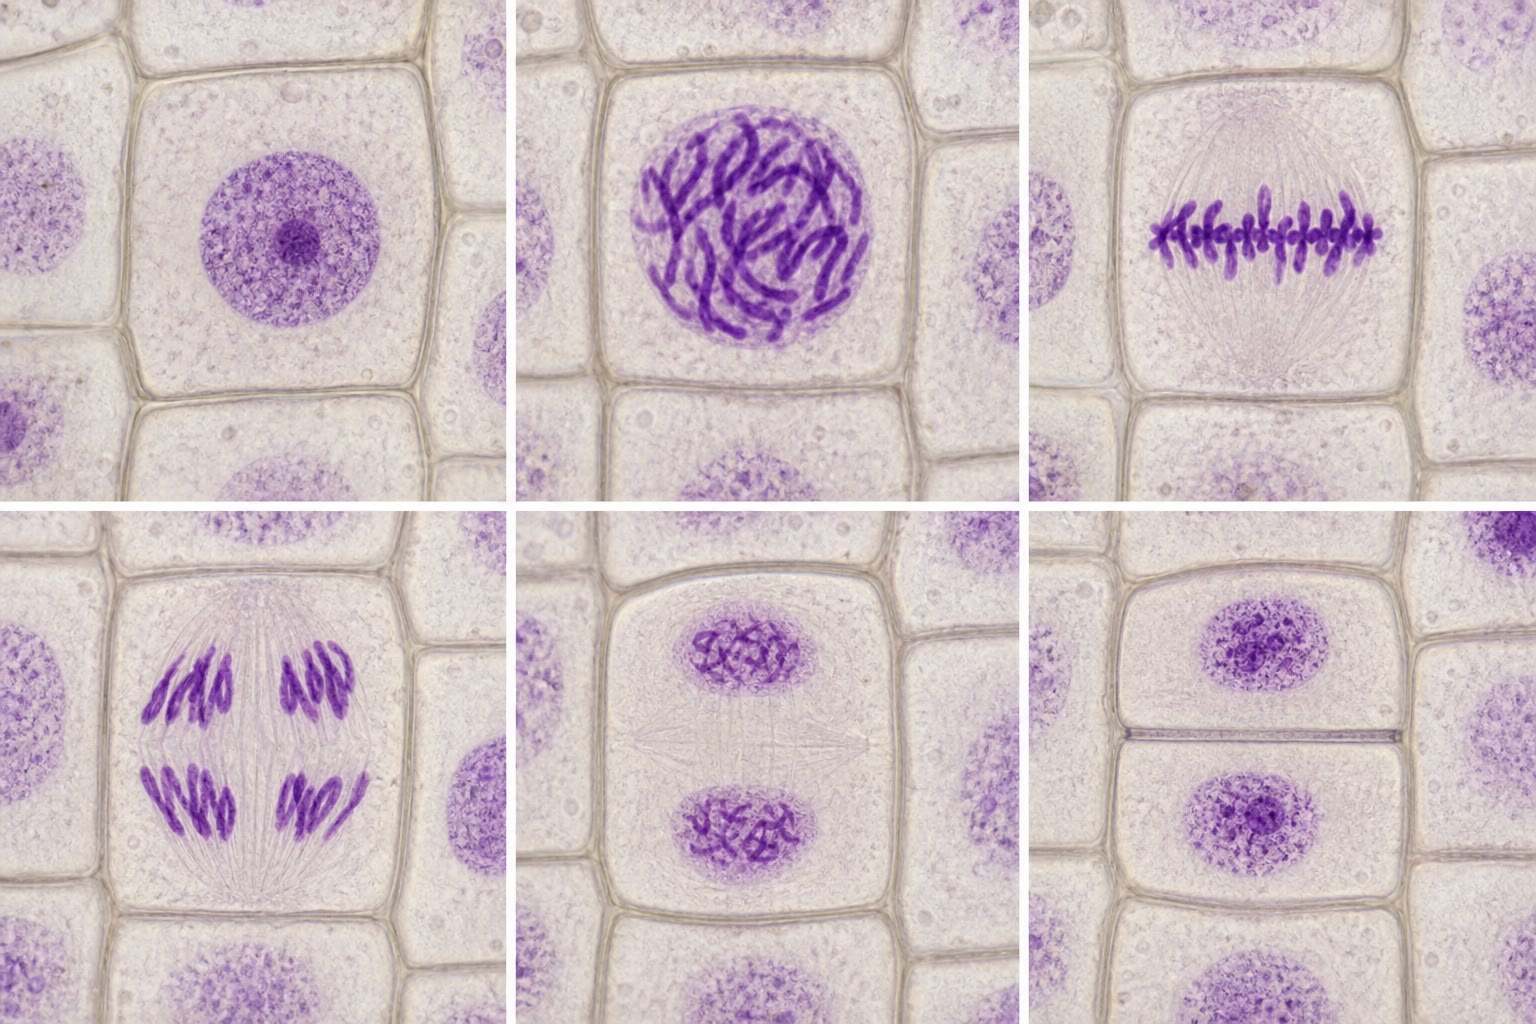
\includegraphics[width=0.9\linewidth]{images/book3/ai/b3-18-mitosis-grid.jpg}

{\small \omterm{def:b1:cell-unit-of-life:cell}{Células} del ápice de una \omterm{def:b1:flowering-plant-organization:organs}{raíz} de cebolla en \omterm{def:b1:replication-mitosis:cycle}{interfase}, profase,
metafase, anafase, telofase y tras la citocinesis, con la pared nueva por el
medio. Los \omterm{def:b1:genomes:genome}{cromosomas} solo son visibles mientras están condensados, de la
profase a la telofase.}
\end{omfigure}

\begin{omfigure}
\begin{tikzpicture}[font=\footnotesize, >=Stealth, line cap=round]
  \foreach \i/\name in {0/profase, 1/metafase, 2/anafase, 3/telofase} {
    \begin{scope}[xshift=\i*3.3cm]
      \draw[thick, omDef!70!black, fill=omDef!5] (0,0) ellipse (1.4 and 1.1);
      \node[anchor=north] at (0,-1.2) {\name};
    \end{scope}
  }
  % prophase: two centrosomes, condensed chromosomes (X shapes) scattered, envelope
  \begin{scope}
    \draw[thick, gray, dashed] (0,0) circle (0.8);
    \foreach \p/\a in {(-0.3,0.25)/30, (0.35,-0.1)/-40, (0.05,-0.45)/80} { \draw[very thick, omThm] \p ++(\a:0.22) -- ++(\a+180:0.44); \draw[very thick, omThm] \p ++(\a+60:0.22) -- ++(\a+240:0.44); }
    \fill[omProp!80!black] (-1.1,0.6) circle (0.07); \fill[omProp!80!black] (1.1,-0.6) circle (0.07);
    \foreach \a in {-30,0,30} { \draw[omProp!60!black] (-1.1,0.6) -- ++(\a-20:0.45); \draw[omProp!60!black] (1.1,-0.6) -- ++(\a+160:0.45); }
  \end{scope}
  % metaphase: spindle pole to pole, chromosomes on the plate
  \begin{scope}[xshift=3.3cm]
    \fill[omProp!80!black] (-1.25,0) circle (0.07); \fill[omProp!80!black] (1.25,0) circle (0.07);
    \foreach \y in {-0.5,-0.25,0,0.25,0.5} { \draw[omProp!60!black] (-1.25,0) -- (0,\y); \draw[omProp!60!black] (1.25,0) -- (0,\y); }
    \foreach \y in {-0.5,-0.17,0.17,0.5} { \draw[very thick, omThm] (-0.12,\y-0.14) -- (0.12,\y+0.14); \draw[very thick, omThm] (-0.12,\y+0.14) -- (0.12,\y-0.14); }
  \end{scope}
  % anaphase: chromatids moving to poles (V shapes)
  \begin{scope}[xshift=6.6cm]
    \fill[omProp!80!black] (-1.25,0) circle (0.07); \fill[omProp!80!black] (1.25,0) circle (0.07);
    \foreach \y in {-0.45,-0.15,0.15,0.45} { \draw[omProp!60!black] (-1.25,0) -- (-0.55,\y); \draw[omProp!60!black] (1.25,0) -- (0.55,\y); \draw[very thick, omThm] (-0.55,\y) -- (-0.35,\y+0.12) (-0.55,\y) -- (-0.35,\y-0.12); \draw[very thick, omThm] (0.55,\y) -- (0.35,\y+0.12) (0.55,\y) -- (0.35,\y-0.12); }
  \end{scope}
  % telophase: two nuclei reforming, cleavage furrow
  \begin{scope}[xshift=9.9cm]
    \draw[thick, gray, dashed] (-0.7,0) circle (0.45); \draw[thick, gray, dashed] (0.7,0) circle (0.45);
    \foreach \x in {-0.8,-0.6,0.6,0.8} { \draw[thick, omThm] (\x,-0.2) -- (\x,0.2); }
    \draw[very thick, omExo!70!black] (0,1.1) -- (0,0.55); \draw[very thick, omExo!70!black] (0,-1.1) -- (0,-0.55);
    \node[font=\scriptsize, omExo!70!black, anchor=south] at (0,1.15) {surco};
  \end{scope}
\end{tikzpicture}

{\small Cuatro etapas de la \omterm{def:b1:replication-mitosis:mitosis}{mitosis} en una \omterm{def:b1:cell-unit-of-life:cell}{célula} animal. Profase: los
\omterm{def:b1:genomes:genome}{cromosomas} se condensan mientras el \omterm{def:b1:replication-mitosis:mitosis}{huso} se forma a partir de los dos
\omterm{def:b1:eukaryotic-cell:cytoskeleton}{centrosomas}. Metafase: cada \omterm{def:b1:genomes:genome}{cromosoma} se sitúa en el ecuador, unido desde
ambos polos. Anafase: las \omterm{def:b1:replication-mitosis:mitosis}{cromátidas} hermanas son separadas. Telofase: dos
núcleos se rehacen y el surco divide la \omterm{def:b1:cell-unit-of-life:cell}{célula}.}
\end{omfigure}

\begin{omfigure}
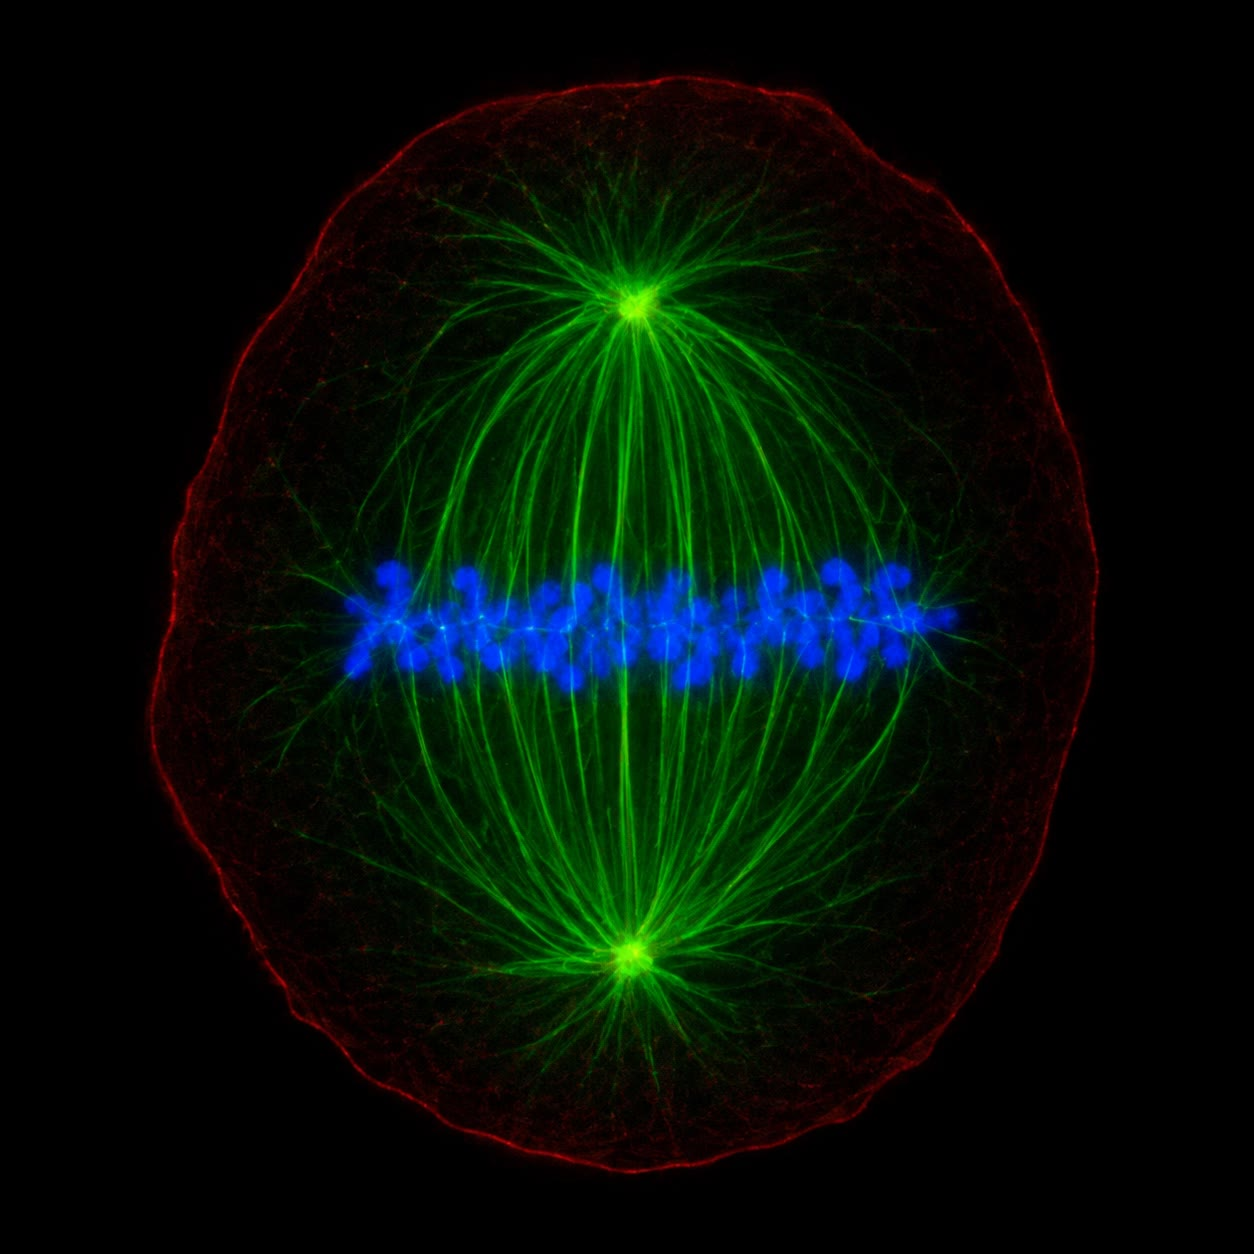
\includegraphics[width=0.4\linewidth]{images/book3/ai/b3-18-mitotic-spindle-fluorescence.jpg}

{\small Una \omterm{def:b1:cell-unit-of-life:cell}{célula} en cultivo en metafase, con sus \omterm{def:b1:eukaryotic-cell:cytoskeleton}{microtúbulos} marcados en
verde y sus \omterm{def:b1:genomes:genome}{cromosomas} en azul: el \omterm{def:b1:replication-mitosis:mitosis}{huso} abarca la \omterm{def:b1:cell-unit-of-life:cell}{célula} de polo a polo y
los \omterm{def:b1:genomes:genome}{cromosomas} forman una placa en su ecuador.}
\end{omfigure}

\begin{proposition}[Qué conserva la mitosis]\label{prop:b1:replication-mitosis:conserves}
La \omterm{def:b1:replication-mitosis:mitosis}{mitosis} es una división que conserva el número de \omterm{def:b1:genomes:genome}{cromosomas}: una \omterm{def:b1:cell-unit-of-life:cell}{célula}
con 2n \omterm{def:b1:genomes:genome}{cromosomas} (46 en el ser humano) da dos \omterm{def:b1:cell-unit-of-life:cell}{células} con 2n. El contenido
de \omterm{def:b1:nucleic-acids:chain}{ADN} pasa de $2q$ (tras la replicación) a $q$ en cada hija; el número de
\omterm{def:b1:genomes:genome}{cromosomas} no cambia nunca, porque un \omterm{def:b1:genomes:genome}{cromosoma} se cuenta por su \omterm{def:b1:genomes:karyotype}{centrómero}
y cada \omterm{def:b1:replication-mitosis:mitosis}{cromátida}, una vez separada, es un \omterm{def:b1:genomes:genome}{cromosoma}. Todas las \omterm{def:b1:cell-unit-of-life:cell}{células} de un
cuerpo son así genéticamente idénticas al óvulo del que descienden, salvo
por las mutaciones que ha introducido la copia. La división que reduce a la
mitad el número de \omterm{def:b1:genomes:genome}{cromosomas}, la meiosis, corresponde al volumen del
segundo año.
\end{proposition}

\begin{method}[Lectura de un experimento sobre el ciclo celular]\label{met:b1:replication-mitosis:reading}
\begin{enumerate}
  \item Mídase el \omterm{def:b1:nucleic-acids:chain}{ADN} por \omterm{def:b1:cell-unit-of-life:cell}{célula} (un colorante cuya fluorescencia sea
        proporcional al \omterm{def:b1:nucleic-acids:chain}{ADN}, \omterm{def:b1:cell-unit-of-life:cell}{célula} a \omterm{def:b1:cell-unit-of-life:cell}{célula}): las \omterm{def:b1:cell-unit-of-life:cell}{células} con $q$ están en
        G$_1$, las que tienen $2q$ en G$_2$ o en M, y las intermedias en S.
        Las fracciones dan las duraciones: la parte del ciclo que ocupa una
        fase es su parte de las \omterm{def:b1:cell-unit-of-life:cell}{células}.
  \item Dese un pulso de \omterm{def:b1:nucleic-acids:nucleotide}{nucleótido} marcado (bromodesoxiuridina): solo lo
        captan las \omterm{def:b1:cell-unit-of-life:cell}{células} en fase S; la fracción marcada es la fracción en
        S, y seguir la marca hasta la \omterm{def:b1:replication-mitosis:mitosis}{mitosis} da la duración de G$_2$.
  \item Cuéntense las figuras de \omterm{def:b1:replication-mitosis:mitosis}{mitosis} en una sección teñida: el
        \emph{índice mitótico}, la fracción de \omterm{def:b1:cell-unit-of-life:cell}{células} en M, es la fracción
        del ciclo que ocupa la M: un \qty{4}{\%} para un ciclo de
        \qty{24}{h} con una \omterm{def:b1:replication-mitosis:mitosis}{mitosis} de una hora.
  \item Bloquéese un paso (un fármaco que despolimerice los \omterm{def:b1:eukaryotic-cell:cytoskeleton}{microtúbulos}
        detiene las \omterm{def:b1:cell-unit-of-life:cell}{células} en metafase; otro que bloquee la síntesis de
        \omterm{def:b1:nucleic-acids:chain}{ADN} las detiene en S) y cuéntese lo que se acumula.
\end{enumerate}
\end{method}

\begin{example}[Recambio]\label{ex:b1:replication-mitosis:turnover}
El \omterm{def:b1:body-plans-tissues:epithelium}{epitelio} del intestino delgado se renueva cada cuatro días, la piel cada
mes y los glóbulos rojos cada cuatro meses a partir de la médula ósea, que
produce dos millones por segundo; una \omterm{def:b1:cell-unit-of-life:cell}{célula} hepática se divide una vez al
año aproximadamente, y una \omterm{def:b1:body-plans-tissues:nervous}{neurona} nunca. Las \omterm{def:b1:cell-unit-of-life:cell}{células} de un tumor han
perdido los \omterm{prop:b1:replication-mitosis:checkpoints}{puntos de control}: se dividen cuando no deberían, toleran
\omterm{def:b1:genomes:genome}{cromosomas} mal repartidos y acumulan las mutaciones que les permiten
dividirse aún más deprisa. La quimioterapia aprovecha la diferencia: los
fármacos que envenenan el \omterm{def:b1:replication-mitosis:mitosis}{huso} o la polimerasa matan a las \omterm{def:b1:cell-unit-of-life:cell}{células} que más
se dividen.
\end{example}

\section{Ejercicios}

\begin{exercise}[$\star$]\label{exo:b1:replication-mitosis:1}
Explíquese por qué en una horquilla una hebra se copia de forma continua y
la otra en fragmentos.
\end{exercise}

\begin{exercise}[$\star$]\label{exo:b1:replication-mitosis:2}
Enumérense las \omterm{def:b1:enzymes:enzyme}{enzimas} y las \omterm{def:b1:proteins:peptide}{proteínas} de una \omterm{def:b1:replication-mitosis:fork}{horquilla de replicación} y la
tarea de cada una.
\end{exercise}

\begin{exercise}[$\star$]\label{exo:b1:replication-mitosis:3}
A partir de la figura del contenido de \omterm{def:b1:nucleic-acids:chain}{ADN}, léanse el contenido de \omterm{def:b1:nucleic-acids:chain}{ADN} en
G$_1$, en G$_2$ y tras la \omterm{def:b1:replication-mitosis:mitosis}{mitosis}, y el número de \omterm{def:b1:genomes:genome}{cromosomas} en cada caso.
\end{exercise}

\begin{exercise}[$\star$]\label{exo:b1:replication-mitosis:4}
Ordénense las etapas de la \omterm{def:b1:replication-mitosis:mitosis}{mitosis} y dese el suceso que define cada una.
\end{exercise}

\begin{exercise}[$\star\star$]\label{exo:b1:replication-mitosis:5}
Calcúlense el número de \omterm{def:b1:replication-mitosis:fork}{fragmentos de Okazaki} que se forman al copiar el
\omterm{def:b1:genomes:genome}{genoma} humano (\num{6.4e9} pares, fragmentos de \qty{150}{}) y el número de
cebadores, de retiradas de cebador y de ligaciones que ello implica.
\end{exercise}

\begin{exercise}[$\star\star$]\label{exo:b1:replication-mitosis:6}
Calcúlese la tasa de error por \omterm{def:b1:genomes:genome}{genoma} humano y por replicación para una
polimerasa sola ($10^{-5}$), con \omterm{prop:b1:replication-mitosis:fidelity}{corrección de pruebas} ($10^{-7}$) y con
reparación de desapareamientos ($10^{-9}$). ¿Cuántas mutaciones da cada caso
por división?
\end{exercise}

\begin{exercise}[$\star\star$]\label{exo:b1:replication-mitosis:7}
Una \omterm{def:b1:cell-unit-of-life:cell}{célula} somática pierde \qty{80}{} \omterm{def:b1:nucleic-acids:nucleotide}{nucleótidos} de \omterm{def:b1:genomes:karyotype}{telómero} por división y
parte de \qty{10}{kb}; deja de dividirse a \qty{5}{kb}. ¿Cuántas divisiones
puede hacer? ¿Por qué necesita telomerasa una \omterm{def:b1:cell-unit-of-life:cell}{célula} cancerosa?
\end{exercise}

\begin{exercise}[$\star\star$]\label{exo:b1:replication-mitosis:8}
Un \omterm{def:b1:body-plans-tissues:tissue}{tejido} tiene el \qty{5}{\%} de sus \omterm{def:b1:cell-unit-of-life:cell}{células} en \omterm{def:b1:replication-mitosis:mitosis}{mitosis} y el \qty{30}{\%}
en fase S; la \omterm{def:b1:replication-mitosis:mitosis}{mitosis} dura una hora. Calcúlense la duración del ciclo y la
de la fase S.
\end{exercise}

\begin{exercise}[$\star\star$]\label{exo:b1:replication-mitosis:9}
Una \omterm{def:b1:cell-unit-of-life:cell}{célula} tiene 2n $= 8$. Dense el número de \omterm{def:b1:genomes:genome}{cromosomas}, el de \omterm{def:b1:replication-mitosis:mitosis}{cromátidas} y
el contenido de \omterm{def:b1:nucleic-acids:chain}{ADN} (en $q$) en G$_1$, en G$_2$, en metafase y en cada hija
tras la telofase.
\end{exercise}

\begin{exercise}[$\star\star\star$]\label{exo:b1:replication-mitosis:10}
\emph{E. coli} necesita \qty{40}{min} para replicar su \omterm{def:b1:genomes:genome}{cromosoma}, pero se
divide cada \qty{20}{min} en un medio rico. Explíquese cómo, y calcúlense
cuántos orígenes y cuántas horquillas contiene una \omterm{def:b1:cell-unit-of-life:cell}{célula} en el momento de
dividirse.
\end{exercise}

\begin{exercise}[$\star\star\star$]\label{exo:b1:replication-mitosis:11}
La colchicina despolimeriza los \omterm{def:b1:eukaryotic-cell:cytoskeleton}{microtúbulos}. Predígase qué le ocurre a una
\omterm{def:b1:cell-unit-of-life:cell}{célula} en división tratada con ella, qué le ocurre a su número de \omterm{def:b1:genomes:genome}{cromosomas}
si después vuelve a entrar en \omterm{def:b1:replication-mitosis:cycle}{interfase}, y por qué se usa el fármaco para
hacer \omterm{def:b1:genomes:karyotype}{cariotipos}.
\end{exercise}

\begin{exercise}[$\star\star\star$]\label{exo:b1:replication-mitosis:12}
``La \omterm{def:b1:replication-mitosis:mitosis}{mitosis} es una copia del \omterm{def:b1:genomes:genome}{genoma} seguida de un recuento.'' Discútase en
un párrafo: qué garantiza la replicación, qué garantiza el \omterm{def:b1:replication-mitosis:mitosis}{huso}, los \omterm{prop:b1:replication-mitosis:checkpoints}{puntos
de control} entre ambos, y qué falla en una \omterm{def:b1:cell-unit-of-life:cell}{célula} que reparte mal un
\omterm{def:b1:genomes:genome}{cromosoma}.
\end{exercise}

\section{Problema: copiar un genoma humano}

\begin{problem}[{Problema de fin de semana --- una fase S de ocho horas:
horquillas cronometradas, orígenes contados, fragmentos y cebadores
sumados, errores calculados y una bacteria comparada, hasta llegar al número
mínimo de orígenes}]
\label{pb:b1:replication-mitosis:1}
Una \omterm{def:b1:cell-unit-of-life:cell}{célula} humana replica $\num{6.4e9}$ \omterm{thm:b1:nucleic-acids:helix}{pares de bases} en una fase S de
\qty{8}{h}. Una horquilla eucariota avanza a \qty{50}{bp/s}; una bacteriana,
a \qty{1000}{bp/s}. Los \omterm{def:b1:replication-mitosis:fork}{fragmentos de Okazaki} son de \qty{150}{} \omterm{def:b1:nucleic-acids:nucleotide}{nucleótidos}
en los eucariotas y de \qty{1500}{} en las bacterias. Cada \omterm{def:b1:nucleic-acids:nucleotide}{nucleótido}
añadido cuesta dos equivalentes de \omterm{def:b1:water-small-molecules:atp}{ATP} (el precursor trifosfato). Tasas de
error por base: $10^{-5}$ para la polimerasa sola, $10^{-7}$ con \omterm{prop:b1:replication-mitosis:fidelity}{corrección
de pruebas} y $10^{-9}$ con reparación de desapareamientos.

\medskip
\noindent\textbf{Parte I --- Horquillas y orígenes.}
\begin{enumerate}
  \item ¿Cuántos \omterm{thm:b1:nucleic-acids:helix}{pares de bases} copia una horquilla en \qty{8}{h}?
  \item Un origen lanza dos horquillas. ¿Cuántos \omterm{thm:b1:nucleic-acids:helix}{pares de bases} copia un
        origen en \qty{8}{h}?
  \item Calcúlese el número mínimo de orígenes necesarios para copiar el
        \omterm{def:b1:genomes:genome}{genoma} en \qty{8}{h} si todos se activan al principio.
  \item Calcúlese la separación media de esos orígenes a lo largo del \omterm{def:b1:nucleic-acids:chain}{ADN},
        en kilobases y en micrómetros.
  \item En realidad los orígenes se activan a lo largo de toda la fase S y
        se usan unos \num{40000}. Calcúlense la separación media y la
        distancia media que recorre realmente una horquilla.
  \item ¿Cuánto tardaría en copiarse el \omterm{def:b1:genomes:genome}{cromosoma} mayor (\qty{250}{Mb})
        desde un único origen situado en su centro?
  \item Explíquese por qué lo que la evolución ajustó para acortar la fase
        S fue el número de orígenes y no la velocidad de las horquillas.
\end{enumerate}

\medskip
\noindent\textbf{Parte II --- Fragmentos y cebadores.}
\begin{enumerate}[resume]
  \item Calcúlese el número de \omterm{def:b1:replication-mitosis:fork}{fragmentos de Okazaki} formados en una fase
        S.
  \item Calcúlese el número de cebadores de \omterm{def:b1:nucleic-acids:chain}{ARN} colocados, incluido uno por
        hebra conductora y por origen.
  \item Calcúlese el número de ligaciones necesarias.
  \item Calcúlense los \omterm{def:b1:nucleic-acids:nucleotide}{nucleótidos} polimerizados en total (las dos hebras
        de todo el \omterm{def:b1:genomes:genome}{genoma}).
  \item Calcúlense los equivalentes de \omterm{def:b1:water-small-molecules:atp}{ATP} gastados en la polimerización y
        el ritmo medio en \omterm{def:b1:water-small-molecules:atp}{ATP} por segundo a lo largo de la fase S.
  \item Compárese con el recambio de \omterm{def:b1:water-small-molecules:atp}{ATP} de una \omterm{def:b1:cell-unit-of-life:cell}{célula} en reposo, de unos
        $10^9$ por segundo: ¿qué fracción de la energía de la \omterm{def:b1:cell-unit-of-life:cell}{célula} va a
        la polimerización?
\end{enumerate}

\medskip
\noindent\textbf{Parte III --- Errores.}
\begin{enumerate}[resume]
  \item Calcúlese el número de errores por fase S para cada una de las tres
        tasas de error.
  \item La secuencia codificante de un \omterm{def:b1:genomes:gene}{gen} mide \qty{1.5}{kb}. Con toda la
        maquinaria, ¿cuál es la probabilidad de que un \omterm{def:b1:genomes:gene}{gen} dado adquiera
        una mutación en una división?
  \item Las \omterm{def:b1:cell-unit-of-life:cell}{células} de una persona sufren unos $10^{16}$ divisiones a lo
        largo de la vida. ¿Cuántas mutaciones en total, a $10^{-9}$? ¿Por
        qué las tolera el cuerpo?
  \item Una mutación inutiliza la reparación de desapareamientos. ¿En qué
        factor sube la tasa de mutación, y qué le hace eso al riesgo de
        cáncer a lo largo de la vida?
\end{enumerate}

\medskip
\noindent\textbf{Parte IV --- La bacteria.}
\emph{E. coli}: \qty{4.6}{Mb}, un origen, dos horquillas.
\begin{enumerate}[resume]
  \item Calcúlese el tiempo de replicar el \omterm{def:b1:genomes:genome}{cromosoma}.
  \item En un medio rico la \omterm{def:b1:cell-unit-of-life:cell}{célula} se divide cada \qty{20}{min}. ¿Cuántas
        rondas de replicación transcurren a la vez, y cuántos orígenes
        lleva una \omterm{def:b1:cell-unit-of-life:cell}{célula} recién nacida?
  \item Calcúlese el número de \omterm{def:b1:replication-mitosis:fork}{fragmentos de Okazaki} por ronda y por
        segundo.
  \item Calcúlense los errores por ronda a $10^{-9}$ y la fracción de
        \omterm{def:b1:cell-unit-of-life:cell}{células} hijas que llevan una mutación nueva.
  \item Un cultivo de $10^9$ \omterm{def:b1:cell-unit-of-life:cell}{células} por mililitro se divide una vez.
        ¿Cuántas mutaciones nuevas aparecen en un mililitro, y cuántas
        alcanzan un \omterm{def:b1:genomes:gene}{gen} dado de \qty{1}{kb}?
  \item Explíquese por qué puede encontrarse resistencia a un antibiótico
        en casi cualquier cultivo grande de una cepa sensible.
  \item Compárense los dos \omterm{def:b1:organism-environment:organism}{organismos}: \omterm{thm:b1:nucleic-acids:helix}{pares de bases}, orígenes, velocidad
        de horquilla, duración de la fase S y el diseño que permite copiar
        el \omterm{def:b1:genomes:genome}{genoma} mayor en un tiempo comparable.
  \item Enúnciese el resultado: el número mínimo de orígenes para una fase
        S humana de \qty{8}{h}, y el número y la separación reales.
\end{enumerate}
\end{problem}
